\documentclass[12pt,]{book}
\usepackage{lmodern}
\usepackage{amssymb,amsmath}
\usepackage{ifxetex,ifluatex}
\usepackage{fixltx2e} % provides \textsubscript
\ifnum 0\ifxetex 1\fi\ifluatex 1\fi=0 % if pdftex
  \usepackage[T1]{fontenc}
  \usepackage[utf8]{inputenc}
\else % if luatex or xelatex
  \ifxetex
    \usepackage{mathspec}
  \else
    \usepackage{fontspec}
  \fi
  \defaultfontfeatures{Ligatures=TeX,Scale=MatchLowercase}
\fi
% use upquote if available, for straight quotes in verbatim environments
\IfFileExists{upquote.sty}{\usepackage{upquote}}{}
% use microtype if available
\IfFileExists{microtype.sty}{%
\usepackage{microtype}
\UseMicrotypeSet[protrusion]{basicmath} % disable protrusion for tt fonts
}{}
\usepackage{hyperref}
\hypersetup{unicode=true,
            pdftitle={Dr.~Duncan Hull},
            pdfborder={0 0 0},
            breaklinks=true}
\urlstyle{same}  % don't use monospace font for urls
\usepackage{natbib}
\bibliographystyle{apalike}
\usepackage{longtable,booktabs}
\usepackage{graphicx,grffile}
\makeatletter
\def\maxwidth{\ifdim\Gin@nat@width>\linewidth\linewidth\else\Gin@nat@width\fi}
\def\maxheight{\ifdim\Gin@nat@height>\textheight\textheight\else\Gin@nat@height\fi}
\makeatother
% Scale images if necessary, so that they will not overflow the page
% margins by default, and it is still possible to overwrite the defaults
% using explicit options in \includegraphics[width, height, ...]{}
\setkeys{Gin}{width=\maxwidth,height=\maxheight,keepaspectratio}
\usepackage[normalem]{ulem}
% avoid problems with \sout in headers with hyperref:
\pdfstringdefDisableCommands{\renewcommand{\sout}{}}
\IfFileExists{parskip.sty}{%
\usepackage{parskip}
}{% else
\setlength{\parindent}{0pt}
\setlength{\parskip}{6pt plus 2pt minus 1pt}
}
\setlength{\emergencystretch}{3em}  % prevent overfull lines
\providecommand{\tightlist}{%
  \setlength{\itemsep}{0pt}\setlength{\parskip}{0pt}}
\setcounter{secnumdepth}{5}
% Redefines (sub)paragraphs to behave more like sections
\ifx\paragraph\undefined\else
\let\oldparagraph\paragraph
\renewcommand{\paragraph}[1]{\oldparagraph{#1}\mbox{}}
\fi
\ifx\subparagraph\undefined\else
\let\oldsubparagraph\subparagraph
\renewcommand{\subparagraph}[1]{\oldsubparagraph{#1}\mbox{}}
\fi

%%% Use protect on footnotes to avoid problems with footnotes in titles
\let\rmarkdownfootnote\footnote%
\def\footnote{\protect\rmarkdownfootnote}

%%% Change title format to be more compact
\usepackage{titling}

% Create subtitle command for use in maketitle
\providecommand{\subtitle}[1]{
  \posttitle{
    \begin{center}\large#1\end{center}
    }
}

\setlength{\droptitle}{-2em}

  \title{Dr.~Duncan Hull}
    \pretitle{\vspace{\droptitle}\centering\huge}
  \posttitle{\par}
    \author{}
    \preauthor{}\postauthor{}
    \date{}
    \predate{}\postdate{}
  
\usepackage{booktabs}

\begin{document}
\maketitle

{
\setcounter{tocdepth}{1}
\tableofcontents
}
\hypertarget{about}{%
\chapter*{About}\label{about}}
\addcontentsline{toc}{chapter}{About}

\begin{center}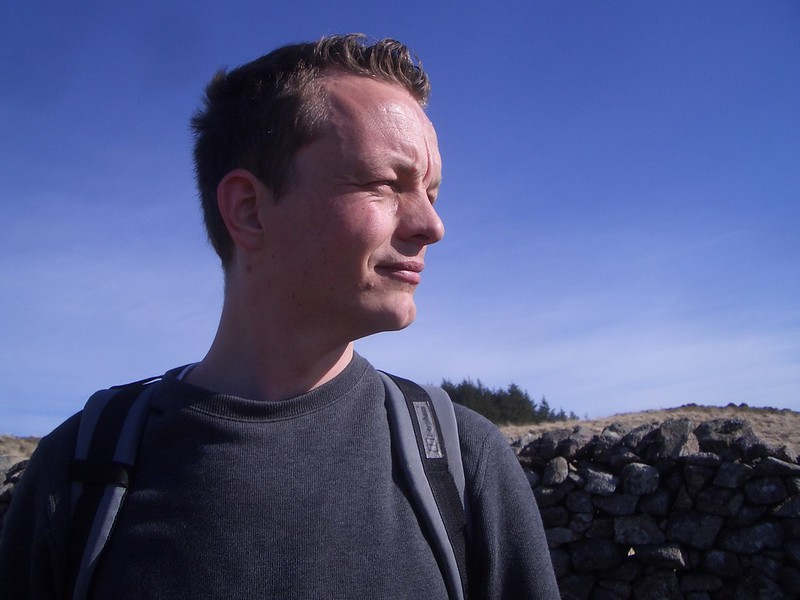
\includegraphics[width=0.25\linewidth]{images/me-blue} \end{center}

Hello, my name is Duncan. I'm a lecturer in the \href{https://www.cs.manchester.ac.uk/}{Department of Computer Science} at the \href{https://www.manchester.ac.uk}{University of Manchester} where I lead the \href{https://www.cs.manchester.ac.uk/study/undergraduate/industrial-experience/}{Industrial Experience (IE)} program. This elective course has over 100 students per year working for 12 months in industry in the penultimate year of their degrees.

I \protect\hyperlink{teaching}{teach} undergraduate courses, supervise tutorials, final year projects and masters projects. I serve as \href{http://studentnet.cs.manchester.ac.uk/ugt/year2/}{second year tutor} and employability tutor. I'm interested in \protect\hyperlink{research}{better teaching and learning methods}, for example using innovative techniques like \protect\hyperlink{vertical-tutoring}{vertical tutoring} and \href{https://www.cs.manchester.ac.uk/connect/business-engagement/industrial-mentoring/}{industrial mentoring} to improve student experience.

If you are an \protect\hyperlink{employers}{employer} who would like to recruit a summer intern, placement student or graduate please \protect\hyperlink{contact}{get in touch}. During term time, we highlight opportunities for students via the \href{https://waggle.cs.manchester.ac.uk/waggle/about}{Wednesday Waggle}. 🐝

\hypertarget{background}{%
\section*{Background}\label{background}}
\addcontentsline{toc}{section}{Background}

My \href{https://uk.linkedin.com/in/duncanhull}{background} is a mixture of Natural Sciences (\href{http://www.plantsciences.manchester.ac.uk/}{Plant Sciences, BSc}), Computer Science (MSc \& PhD) and software engineering. I've worked as a consultant and software developer for various organisations including \href{https://en.wikipedia.org/wiki/BBC_Monitoring}{BBC Monitoring}, the \href{https://en.wikipedia.org/wiki/Ford_Motor_Company}{Ford Motor Company} and the \href{https://en.wikipedia.org/wiki/National_Health_Service}{National Health Service} (NHS). While working on the \href{https://en.wikipedia.org/wiki/Apache_Taverna}{Apache Taverna}, \href{https://en.wikipedia.org/wiki/MyGrid}{myGrid} and \href{http://www.nactem.ac.uk/pathtext/}{Refine project} I completed a \href{https://ethos.bl.uk/OrderDetails.do?uin=uk.bl.ethos.497578}{PhD} and \href{https://en.wikipedia.org/wiki/Postdoctoral_researcher}{postdoc} in \href{https://en.wikipedia.org/wiki/Bioinformatics}{Bioinformatics} at the University of Manchester. More recently, I was employed as a software engineer of a biochemical database (\href{https://www.ebi.ac.uk/chebi/}{Chemical Entities of Biological Interest: ChEBI}) in Cambridge, UK at the European Bioinformatics Institute (\href{https://www.ebi.ac.uk}{ebi.ac.uk}). 🇪🇺

I have taught english, maths, science and engineering from primary to postgraduate level and beyond. This has included work with primary \& secondary school children (\href{https://en.wikipedia.org/wiki/K\%E2\%80\%9312}{K--12}), undergraduates \& postgraduates in the UK, India and America. 🇬🇧🇮🇳🇺🇸

\hypertarget{tools}{%
\section*{Tools}\label{tools}}
\addcontentsline{toc}{section}{Tools}

This website is written in \href{https://rmarkdown.rstudio.com/}{R markdown} and built using \href{https://bookdown.org}{bookdown}, \href{https://www.gitbook.com}{gitbook}, \href{https://en.wikipedia.org/wiki/Knitr}{knitr}, \href{https://en.wikipedia.org/wiki/LaTeX}{LaTeX}, \href{https://pandoc.org/}{pandoc}, \href{https://code.visualstudio.com/}{Visual Studio Code} and \href{https://www.rstudio.com/}{RStudio}. The \href{https://github.com/dullhunk/hulled}{source is available on github}. It could have (should have?) been built using \href{https://bookdown.org/yihui/blogdown/}{blogdown} and \href{https://gohugo.io}{Hugo}, but bookdown was chosen because it is much \sout{less bloated} easier to use. 🔨

\hypertarget{teaching}{%
\chapter{Students}\label{teaching}}

I teach 🎓 on a variety of undergraduate and postgraduate courses including:

\hypertarget{all-years-debug-your-cv}{%
\section{All years: debug your CV}\label{all-years-debug-your-cv}}

\begin{itemize}
\tightlist
\item
  You can drop-in to my weekly one-to-one CV clinics for Computer Science students in LF25 during term-time. Whatever stage you are at, it is a good idea to \textbf{debug} your CV, LinkedIn, job search, life etc before you show it to a potential employer. These sesions are open to undergraduate (BSc, BEng) and postgradautes (MSc and PhD). If you haven't written a CV, résumé or LinkedIn profile before, you might find the \emph{Debug your CV} guide useful at \href{http://git.io/mycv}{git.io/mycv}. Outside of term time, you'll need to book an appointment.
\end{itemize}

\hypertarget{first-year}{%
\section{First year}\label{first-year}}

\begin{itemize}
\tightlist
\item
  \href{https://studentnet.cs.manchester.ac.uk/ugt/COMP10120/syllabus/}{First year team projects: COMP101} led by \href{http://www.cs.man.ac.uk/~sattler/}{Ulrike Sattler}
\item
  Mentoring one group of six first year students
\item
  Organise first year guest lectures, which mostly run in the second semester, February to May
\end{itemize}

\hypertarget{second-year}{%
\section{Second year}\label{second-year}}

\begin{itemize}
\tightlist
\item
  \href{https://studentnet.cs.manchester.ac.uk/ugt/COMP23311/syllabus/}{Second year software engineering: COMP23311} led by \href{http://www.cs.man.ac.uk/~embury/}{Suzanne Embury}
\item
  Lab organiser for the \href{https://www.cs.manchester.ac.uk/connect/business-engagement/industrial-mentoring/}{software engineering mentoring program}
\item
  Leading second year tutorials COMP2CARS and being a second year tutor to a group of six students
\end{itemize}

\hypertarget{penultimate-year}{%
\section{Penultimate year}\label{penultimate-year}}

\begin{itemize}
\tightlist
\item
  Course leader for ``with industrial experience'' (IE), an elective and intercalated year in industry.
\end{itemize}

\hypertarget{final-year}{%
\section{Final year}\label{final-year}}

\begin{itemize}
\tightlist
\item
  Supervising final year educational projects based in secondary schools in Manchester, see \href{https://git.io/computinged}{git.io/computinged}.
\end{itemize}

\hypertarget{masters}{%
\section{Masters}\label{masters}}

\begin{itemize}
\tightlist
\item
  Supervising \href{https://www.cs.manchester.ac.uk/study/masters/}{Master of Science} projects in Computer Science and Data Science. This often includes research using Wikipedia, Wikdiata and chatbots. 🤖
\end{itemize}

\hypertarget{extra-curricular}{%
\section{Extra-curricular}\label{extra-curricular}}

\begin{itemize}
\tightlist
\item
  Organise, facilitate and promote extra-curricular activities, usually off-timetable (for example Wednesday afternoons, evenings and weekends). I'm proud to have served as a judge of the fantastic \href{https://www.studenthack.com}{studenthack.com} and \href{https://greatunihack.com}{greatunihack.com} since they started in 2014. These \href{https://medium.com/tfogo/hackathons-are-for-beginners-77a9c9c0e000}{hackathons} are organised by \href{https://www.unicsmcr.com/}{UniCS}, a student-led tech society formerly known as HackSoc and CSSoc.
\end{itemize}

\hypertarget{employers}{%
\chapter{Employers}\label{employers}}

We work with a wide range of employers from the tiniest startup to the largest multi-national corporations, and are always looking for more organisations that can offer our students a stimulating environment to work in. According to \href{https://www.highfliers.co.uk}{highfliers.co.uk}, the University of Manchester is one of the most targeted Universities in the UK by the \href{https://www.top100graduateemployers.com}{Times Top 100 Graduate Employers}. We're keen to do better, for example, by engaging more with new employers, especially those in Manchester (see \href{https://git.io/manc}{git.io/manc}).

\hypertarget{recruiting-students}{%
\section{Recruiting students}\label{recruiting-students}}

If you are recruiting computer scientists and software engineers as a summer interns, placement students or as graduates please get in touch with me or \href{https://uk.linkedin.com/in/mabel-yau}{Mabel Yau} (careers and placements officer). We typically have around 250 undergraduate students graduating annually, alongside a smaller number of Masters and PhD students.

If you are looking to recruit students from related degree disciplines like \href{https://www.physics.manchester.ac.uk/}{Physics}, \href{https://www.maths.manchester.ac.uk/}{Maths}, \href{https://www.chemistry.manchester.ac.uk/}{Chemistry}, \href{https://www.mace.manchester.ac.uk/}{MACE} and \href{https://www.eee.manchester.ac.uk/}{EEE} you should talk to the Careers Service centrally at \href{http://www.careers.manchester.ac.uk/}{careers.manchester.ac.uk}

\hypertarget{careers-fairs}{%
\section{Careers fairs}\label{careers-fairs}}

Our annual Computer Science careers fair is held the Kilburn building in autumn, we typically have around 30 employers exhibited over two days.

We also run drop-in sessions where employers can come in and set up a stand in the foyer to talk to students informally on their way to and from lectures, usually during lunch in \href{https://www.manchester.ac.uk/discover/key-dates/}{term time}. If you're interested in exhibiting at either of these, please \protect\hyperlink{contact}{contact the careers and placements officer Mabel Yau}.

The central careers service also organises

\begin{itemize}
\item
  the big careers fair in \href{https://www.manchestercentral.co.uk/}{Manchester Central} every autumn, see the \href{http://www.careers.manchester.ac.uk/events/bigcareersfair/}{Big Careers Fair}
\item
  a smaller careers fair in Fallowfield \href{http://www.sport.manchester.ac.uk/facilities/armitage/}{Armitage centre} in May
\end{itemize}

\hypertarget{industry-club}{%
\section{Industry Club}\label{industry-club}}

Employers are welcome to join our industry club mailing list by sending an email to \href{mailto:listserv@listserv.manchester.ac.uk}{\nolinkurl{listserv@listserv.manchester.ac.uk}} with the the text \textbf{subscribe cs-industryclub yourfirstname yoursecondname} in the body of your message.

You will receive two to three updates per year and an invitation to our industry club meetings which usually happen every year. We promise not to spam you or sell your details on to third parties.

\hypertarget{the-wednesday-waggle}{%
\section{The Wednesday Waggle}\label{the-wednesday-waggle}}

During term time, we highlight events and vacancies from a \href{http://dullhunk.github.io/where-can-I-look-for-jobs.html}{wide range of sources} to students via the \href{https://waggle.cs.manchester.ac.uk/waggle/about}{Wednesday Waggle}. If you have vacancies or events you would like our students to know about, \protect\hyperlink{contact}{get in touch}.

\hypertarget{research}{%
\chapter{Research}\label{research}}

My research interests are in Computer Science Education (CSE) and \href{https://en.wikipedia.org/wiki/Pedagogy}{pedagogy}. I am particularly interested in better \href{https://www.manchester.ac.uk/study/undergraduate/teaching-learning/}{teaching and learning methods} that prepare students for the wide range of careers they go onto after graduation. This includes ``hard'' technical and ``soft'' non-technical skills.

\textbackslash{}begin\{figure\}

\{\centering 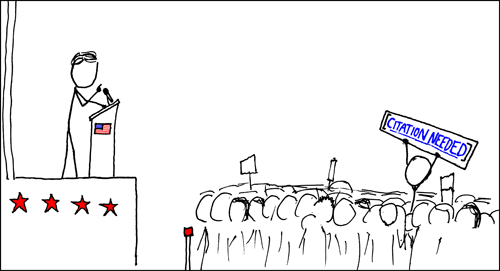
\includegraphics[width=0.7\linewidth]{images/wikipedian_protester}

\}

\textbackslash{}caption\{Many educational practices are not backed up by good evidence that they actually work. More evidence (citations) is needed to support some of the claims made about pedagogy and teaching Computer Science. This \emph{Wikipedian Protester} cartoon is by \href{https://en.wikipedia.org/wiki/Randall_Munroe}{Randall Munroe} at \href{https://xkcd.com/285/}{xkcd.com/285} Creative Commons Attribution-NonCommercial 2.5 License\}\label{fig:unnamed-chunk-2}
\textbackslash{}end\{figure\}

\hypertarget{sigcse}{%
\section{SIGCSE}\label{sigcse}}

In the UK we have only been teaching Computer Science to undergraduates \href{http://www.bbc.co.uk/manchester/content/articles/2005/11/07/baby_computer_40_interview_feature.shtml}{for 50 short years}, so there's lots of open questions about how to teach the practical and theoretical aspects of the subject.

\begin{itemize}
\tightlist
\item
  I'm an active member of the \href{https://en.wikipedia.org/wiki/Association_for_Computing_Machinery}{Association for Computing Machinery} (ACM) Special Interest Group (SIG) in Computer Science Education (\href{https://sigcse.org}{SIGCSE.org}).
\item
  As part of that I founded and chair a \href{https://duncan.hull.name/2019/07/17/sigcse-journal-club/}{journal club} for educators in Manchester, if you'd like to join us, subscribe to the mailing list by emailing \href{mailto:listserv@listserv.manchester.ac.uk}{\nolinkurl{listserv@listserv.manchester.ac.uk}} with the text \textbf{subscribe sigcse-journal-club yourfirstname yoursecondname} in the body of your message
\item
  I'm serving on the program committee for \href{http://community.dur.ac.uk/cep.conference}{Computing Education \& Practice (CEP)} at Durham University.
\end{itemize}

\hypertarget{code-club}{%
\section{Code Club}\label{code-club}}

I lead an after school \href{https://codeclub.org}{CodeClub}, part of a global network of free coding clubs for 9--13 year olds. The aim is to have fun using scratch, python and other interesting technology we can get our hands on including \href{https://www.raspberrypi.org/}{Raspberry Pi}, \href{https://microbit.org/}{Micro:bits}, \href{https://www.lego.com/en-gb/themes/mindstorms}{LEGO® MINDSTORMS®}, \href{https://www.oculus.com}{Oculus Rift}, \href{https://sonic-pi.net/}{Sonic Pi} and \href{http://www.codebug.org.uk/}{CodeBug} etc.

\hypertarget{wikipedia}{%
\section{Wikipedia}\label{wikipedia}}

Wikipedia (and its sister project \href{https://www.wikidata.org}{wikidata.org}) are great tools for improving digital skills and communication skills, regardless the learners level of computer literacy. As an experience and long serving editor of Wikipedia since 2004, I organise and participate in \href{https://en.wikipedia.org/wiki/Edit-a-thon}{edit-a-thons} which recruit and train new Wikipedia editors in collaboration with other volunteers. More information at:

\begin{itemize}
\tightlist
\item
  \href{https://wiki-loves-scientists.org.uk/}{wiki-loves-scientists.org.uk}
\item
  \href{https://en.wikipedia.org/wiki/User:Duncan.Hull}{en.wikipedia.org/wiki/User:Duncan.Hull}
\end{itemize}

\hypertarget{informal-publications}{%
\section{Informal publications}\label{informal-publications}}

Informal publications can be found on my sporadically updated blog

\begin{itemize}
\tightlist
\item
  \href{https://duncan.hull.name/lablog/}{duncan.hull.name/lablog}
\end{itemize}

\hypertarget{formal-publications}{%
\section{Formal publications}\label{formal-publications}}

Formal peer-reviewed publications can be found on DBLP, ORCID and Google Scholar\ldots{}

\begin{itemize}
\tightlist
\item
  \href{https://dblp.org/pid/h/DuncanHull}{dblp.org/pid/h/DuncanHull}
\item
  \href{https://orcid.org/0000-0003-2387-503X}{orcid.org/0000-0003-2387-503X}
\item
  \href{https://scholar.google.com/citations?user=iDJ-t7IAAAAJ}{scholar.google.com/citations?user=iDJ-t7IAAAAJ}
\end{itemize}

\ldots{}and even wikidata:

\begin{itemize}
\tightlist
\item
  \href{https://www.wikidata.org/wiki/Q47012855}{wikidata.org/wiki/Q47012855}
\end{itemize}

\hypertarget{vertical-tutoring}{%
\chapter{Vertical tutoring}\label{vertical-tutoring}}

Starting in September 2019, I am leading an experiment with a vertical tutoring system for undergraduate students. The idea is fairly widespread in secondary education (see \href{https://www.verticaltutoring.org/}{verticaltutoring.org}), but as far as we know has not been used fully in higher education.

Extending the idea of Peer Assisted Study Sessions (PASS) \href{http://www.pass.manchester.ac.uk}{pass.manchester.ac.uk}, vertical tutoring creates tutorial groups with a representative from \emph{one of each} of several years and combined with alumni. For example, a vertical tutor group could contain:

\begin{itemize}
\tightlist
\item
  One first year student
\item
  One second year student
\item
  One student out on placement
\item
  One final year student
\item
  One member of our alumni
\end{itemize}

\hypertarget{full-stack-mentoring}{%
\section{Full stack mentoring}\label{full-stack-mentoring}}

This is a work in progress. Watch this space for updates!

\hypertarget{contact}{%
\chapter{Contact}\label{contact}}

You can contact us using the the details below

\hypertarget{office}{%
\section{Office}\label{office}}

\textbf{Dr.~Duncan Hull, Lecturer} 👨‍💻

\begin{itemize}
\tightlist
\item
  🏢 Room LF25, Kilburn Building: \href{http://bit.ly/directions-to-kilburn-building}{bit.ly/directions-to-kilburn-building}
\item
  📥 email: \href{mailto:duncan.hull@manchester.ac.uk}{\nolinkurl{duncan.hull@manchester.ac.uk}}
\item
  ☎️ telephone: +44 161 275 6186
\item
  🌐 \href{https://uk.linkedin.com/in/duncanhull}{linkedin.com/in/duncanhull}
\end{itemize}

\textbf{Mabel Yau, Careers and placements officer} 👩‍💻

\begin{itemize}
\tightlist
\item
  🏢 Room LF26, Kilburn Building:
\item
  📥 email: \href{mailto:mabel.yau@manchester.ac.uk}{\nolinkurl{mabel.yau@manchester.ac.uk}}
\item
  ☎️ telephone: +44 161 275 6140
\item
  🌐 \href{https://uk.linkedin.com/in/mabel-yau}{linkedin.com/in/mabel-yau}
\end{itemize}

\hypertarget{elsewhere}{%
\section{Elsewhere}\label{elsewhere}}

I can also be found on:

\begin{itemize}
\tightlist
\item
  Slack: search for ``Duncan Hull'' or my work email
\item
  Skype: search for ``duncanhull''
\item
  Blog: \href{https://duncan.hull.name}{duncan.hull.name}
\item
  Github: \href{https://github.com/dullhunk}{github.com/dullhunk}
\item
  Twitter: \href{https://twitter.com/dullhunk}{twitter.com/dullhunk}
\end{itemize}

\hypertarget{postal-address}{%
\section{Postal address}\label{postal-address}}

Send post 🐌 to :

Dr.~Duncan Hull\\
Department of Computer Science\\
Kilburn Building\\
The University of Manchester\\
Oxford Road\\
Manchester\\
M13 9PL

\bibliography{hulld.bib}


\end{document}
